\label{chap:machine_model}

In this section, we will describe the abstract architecture upon which our PDP protocol operates in order to motivate the current and future use-cases for our protocol. Additionally, we will discuss how different components operate in the system in order to give the reader an intuition of the underlying operation.

\begin{figure}
    \centering
        \centering
        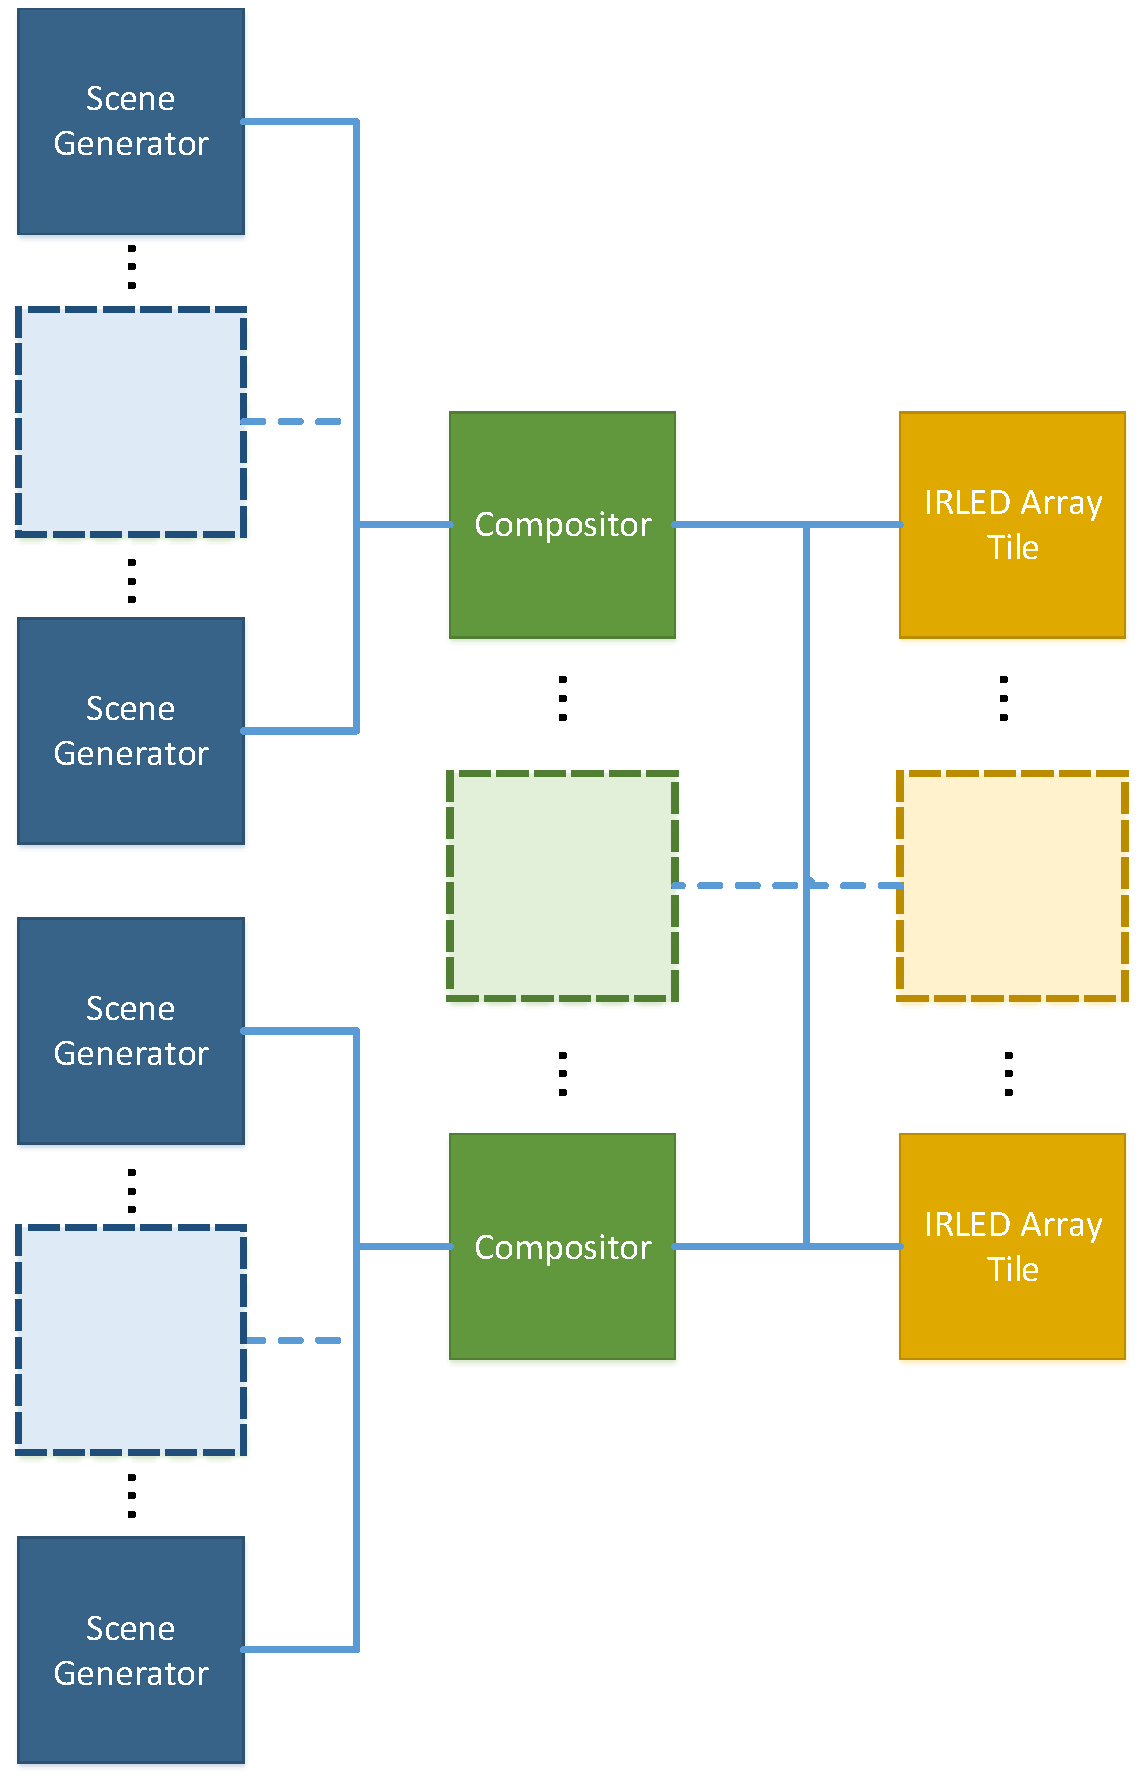
\includegraphics[width=0.75\textwidth]{fig/amm.pdf}
        \caption{Abstract Machine Model of our PDP architecture with 1-to-N relationships between components}
        \label{fig:amm}
\end{figure}

\begin{figure}
        \centering
        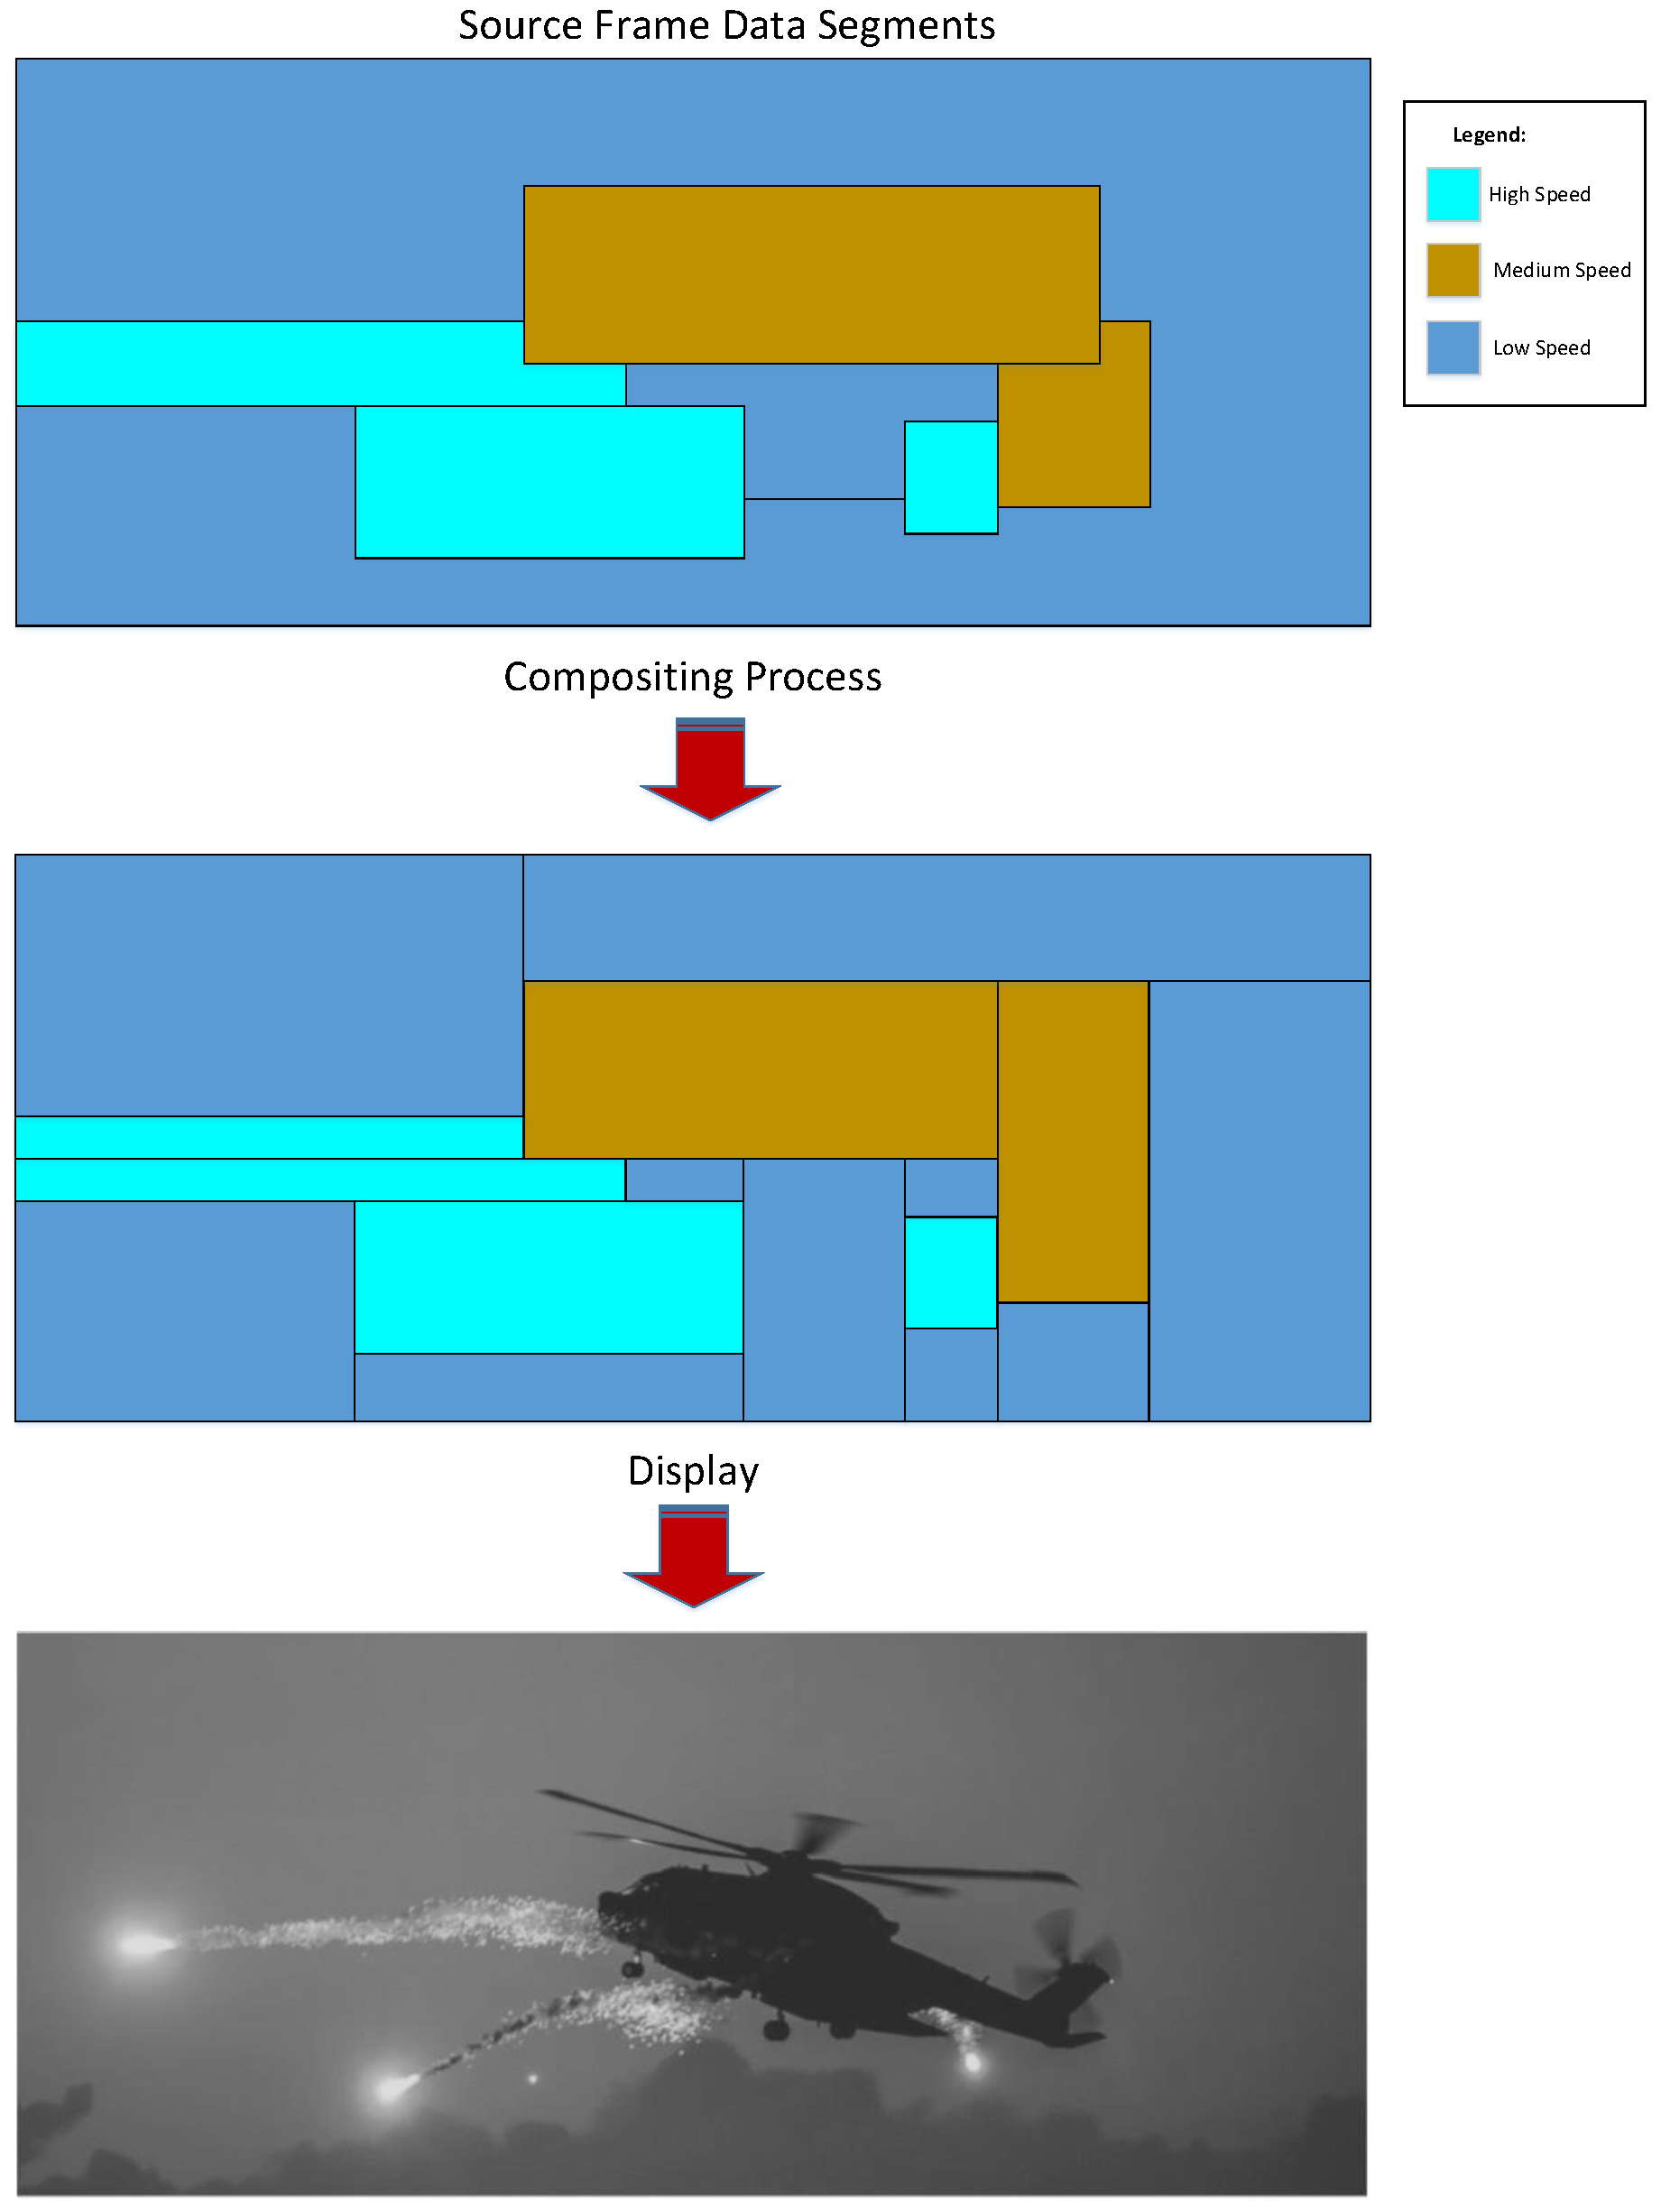
\includegraphics[width=1.0\textwidth]{fig/compositing.pdf}
        \caption{Compositing Process Example}
        \label{fig:compositing}
    \caption{Abstract Machine Model and Compositing Process}
\end{figure}


Traditional IRLED display systems are typically composed of three components as part of the display: scene generation, non-uniformity correction, and the actual display of InfraRed with sensors used to capture data. We propose an Abstract Machine Model (AMM) to capture these three components as shown in figure \ref{fig:amm}. This AMM separates the system operation of an IRLED system into three main components as well: scene generation, compositing, and display on IRLED array tiles with links between each component. The relationship between these components remains abstracted in such a way that hardware components may be scaled to fit demand. At its most basic, a single scene generator, compositor, and IRLED array tile may be used. For higher speed requirements, hardware components may be mapped as needed. The links between components in the system utilize the PDP protocol for communication, data-transfer, and synchronization. The compositing component differs from a traditional IRLED system in that it is responsible for taking imagery from many sources, possibly at different frame rates, and combining them into a single image for transmission to IRLED array tiles. This process is briefly shown in figure \ref{fig:compositing}. During the compositing process frame segments are ranked to determine which to send at high speeds, and which to send at low speeds for intelligent bandwidth utilization. Once segmented and ranked into non-overlapping speed classes, frame segments are transmits at the necessary rate.

For example consider the simple case, that of a single scene generator. In this case, the compositor will receive data from a single source. As frame data is received, a differencing algorithm must be employed to determine how to segment the overall frame for optimal data transfer based off of the rate of change of individual portions of the frame relative to the prior frame. Portions that rapidly change will be sent more often than portions that change slowly in order to maximize bandwidth for high-speed transfer of {\it hot} portions of an image. This consequently also has the effect of improving the performance of the analog chain of display devices by allowing for devices to reserve more time to drive rapidly changing portions of a display over portions of the display changing relatively slowly.
